\documentclass[11pt, oneside]{article}
\usepackage[margin=1in,letterpaper]{geometry}
\usepackage{times}
\usepackage{graphicx}
\usepackage{amssymb,amsmath,mathtools}
\usepackage{array}
\usepackage{longtable}
\usepackage{color}
\usepackage[T1]{fontenc}
\usepackage{sectsty}
\usepackage[normalem]{ulem} % \uline: line-breakable underline for long underlined phrases
\usepackage{tikz}
\usetikzlibrary{decorations.pathmorphing,decorations.markings,decorations.pathreplacing,calc,patterns,arrows.meta,shapes.geometric}
\usepackage{float}
\usepackage{pgfplots}
\pgfplotsset{compat=1.17}
\sectionfont{\fontsize{12}{12}\selectfont}
\subsectionfont{\fontsize{11}{11}\selectfont}
\subsubsectionfont{\normalsize\itshape\mdseries}

\renewcommand\labelitemi{{\boldmath$\cdot$}}
% NOTE: dots at every level; the handwritten dashes are set explicitly with \item[--].
\renewcommand\labelitemii{\labelitemi}
\renewcommand\labelitemiii{\labelitemi}
\renewcommand\labelitemiv{\labelitemi}

%%%%%%%%%%%%%%%%%%%%%%%%%%%%%%%%%%%%%
% Notation: symbols follow ../variables_master.tex. Renames that apply existing instructor decisions (each also marked
% at first use):
%   - molecular energies U, U_e, U_v, U_r -> script E, E_e, E_v, E_r (D95); rotation rate omega -> omega_rot (D96);
%     rotational quantum number l -> J (D98); vibrational quantum number (handwritten nu_k, Liou's upsilon_k) ->
%     n_vib,k and the mode's angular frequency omega_k -> omega_vib,k (D96, D99); vibration-level labels
%     nu_0, nu_1, nu_2 in the potential-energy sketch -> n_vib = 0, 1, 2 (D99);
%   - damping coefficient gamma (and gamma_0) -> nu (nu_0) (D9: gamma is reserved for the propagation constant; L1 uses
%     nu for the same oscillator damping);
%   - wavenumbers K, K_0 -> k, k_0 and Boltzmann K_B -> k_B (D14);
%   - phase velocity v_p -> u_p (D15, as in Ulaby & Long); group velocity v_g -> u_g (same pattern);
%   - transitions T_1, T_2 -> script T_1, T_2 (D19: T is temperature only; flagged as D105);
%   - energy difference Delta E -> Delta script E (D95; F8 promoted to D100).
% Instructor decisions (2026-09-30, master table D100--D116): renamed (resolved): principal quantum number n -> n_el
% (D101); Doppler absorption coefficient kappa_d -> kappa_a,D (D111); line-center wavenumber k_0 -> k_line (D113).
% Kept (approved): the rest of D100--D116, including T_0 = 273 K as handwritten (D116); D110 approved with a
% sentence stating the two normalizations of S.
% Not triggered in this lecture (no optical depth, phase function, mu = cos theta, or Stefan--Boltzmann constant): F2,
% F3, F6, F11.
% Main reference checks: Liou (2002), Sec. 1.3 (pp. 14-25), Eqs. 1.3.1-1.3.18, Figs. 1.9, 1.11; Sec. 3.2 (pp. 70-73),
% Figs. 3.3, 3.4; App. D (pp. 529-532), Eqs. D.10-D.18, Fig. D.1. Ulaby & Long (2014), Sec. 8-2 (pp. 328-333),
% Eqs. 8.9-8.17.
%%%%%%%%%%%%%%%%%%%%%%%%%%%%%%%%%%%%%

\title{Ge 158 Lecture 11: Atmospheric Absorption and Emission}
\author{Brent Minchew}
\date{}

\setlength{\emergencystretch}{1.5em}
\renewcommand{\topfraction}{0.85}
\renewcommand{\textfraction}{0.1}
\renewcommand{\floatpagefraction}{0.75}
\begin{document}
\maketitle

\noindent\underline{\textbf{Topics covered}}
\begin{itemize}
	\item Atmospheric energy states
	\begin{itemize}
		\item[--] Vibrational energy
		\item[--] Electronic energy
		\item[--] Synthesis of energy states
	\end{itemize}
	\item Broadening mechanisms w/ emphasis on pressure broadening
\end{itemize}

%%%%%%%%%%%%%%%%%%%%%%%%%%%%%%%%%%%%%
\section{Absorption and emission by gases (cont.\ from prev.\ lecture)}
\label{s:recap}

\begin{itemize}
	\item Recall that this is a very high-level discussion of absorption and emission by atmospheric gases
	\begin{itemize}
		\item[$\rightarrow$] Students interested in a deeper dive should look into 12.315/12.815
	\end{itemize}
	% NOTE: the handwritten U, U_e, U_v, U_r are written script E (master table D95); l is written J (D98); omega is
	% written omega_rot (D96). Checked against U&L 2014, Eq. 8.9 (p. 328) and Liou 2002, Eqs. 1.3.5-1.3.6 (p. 18).
	\item Recall from prev.\ lecture:\\
	Total energy $\mathcal{E}$ of isolated molecule consists of 3 energy states
	\begin{equation}
		\label{e:E}
		\mathcal{E} = \mathcal{E}_\mathrm{e} + \mathcal{E}_\mathrm{v} + \mathcal{E}_\mathrm{r},
	\end{equation}
	\begin{itemize}
		\item[] $\mathcal{E}_\mathrm{e} \equiv$ electronic energy $\rightarrow$ electron energy levels in individual atoms,
		\item[] $\mathcal{E}_\mathrm{v} \equiv$ vibrational energy $\rightarrow$ displacement between 2 or more nuclei,
		\item[] $\mathcal{E}_\mathrm{r} \equiv$ rotational energy $\rightarrow$ rotation of molecule.
	\end{itemize}
	% NOTE: the handwritten mark before "Key point" is read as a star (low confidence; possibly an asterisk).
	$\bigstar$ Key point: energy states are quantized
	\begin{itemize}
		\item[--] Rotational energy covered last lecture:
		\begin{equation}
			\label{e:Er}
			\mathcal{E}_\mathrm{r} = \frac{\omega_\mathrm{rot}\hbar\sqrt{J(J+1)}}{2}, \qquad
			\begin{aligned}
				&\hbar \equiv \text{(reduced) Planck const},\\
				&J \equiv \text{nonnegative integer ``rotational quantum number''}.
			\end{aligned}
		\end{equation}
	\end{itemize}
\end{itemize}

%%%%%%%%%%%%%%%%%%%%%%%%%%%%%%%%%%%%%
% NOTE: subsection heading added; it is the handwritten bullet "Vibrational energy U_v" (page L2).
\subsection{Vibrational energy $\mathcal{E}_\mathrm{v}$}
\label{s:vib}

\begin{itemize}
	\item[--] Distance between atomic nuclei is influenced by absorption and emission of EM radiation
	% NOTE: added "(Figure~\ref{f:vib})".
	\item[--] Basic process (Figure~\ref{f:vib})

\begin{figure}[!htbp]
	\centering
	% Reproduces the handwritten sketch (page L2), element by element: two shaded atoms joined by a spring, - above the
	% left atom and + above the right; a wave labeled "EM radiation" to the right, with its arrowhead at its left end
	% pointing at the + atom; below the atoms a rightward arrow (under -) and a leftward arrow (under +); the text
	% "positive side of dipole is pushed by EM radiation and negative side is pulled, causing nuclei to move closer to
	% one another". To the right: two open circles joined by a spring; below, a leftward arrow (under the left atom)
	% and a rightward arrow (under the right atom); the text "nuclei are both positively charged => repel". A curved
	% arrow with arrowheads at both ends, bowed downward, links the two texts, above the conclusion "=> EM radiation
	% pushes nuclei together, like charges repel => vibration". (No "1)", "2)" labels, unlike Lecture 10.)
	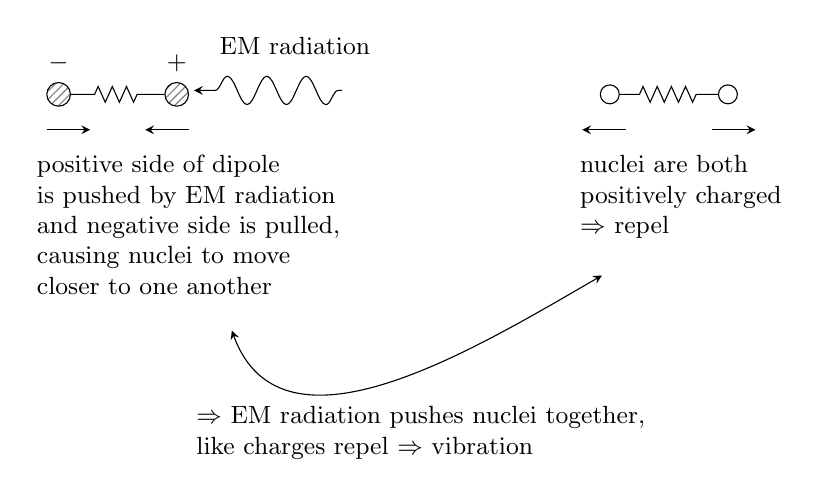
\begin{tikzpicture}[>=stealth, font=\small]
		\tikzset{atom/.style={draw, circle, minimum size=0.3cm, inner sep=0pt, pattern=north east lines, pattern color=gray}}
		\tikzset{oatom/.style={draw, circle, minimum size=0.24cm, inner sep=0pt}}
		\node[atom] (a1) at (0,0) {};
		\node[atom] (b1) at (1.5,0) {};
		\draw[decorate, decoration={zigzag, amplitude=0.1cm, segment length=0.18cm, pre length=0.3cm, post length=0.3cm}] (a1) -- (b1);
		\node at (0,0.4) {$-$};
		\node at (1.5,0.4) {$+$};
		\draw[->, decorate, decoration={snake, amplitude=0.18cm, segment length=0.5cm, pre length=0.05cm, post length=0.12cm}] (3.6,0.05) -- (1.72,0.05);
		\node at (3.0,0.62) {EM radiation};
		\draw[->] (-0.15,-0.45) -- (0.4,-0.45);
		\draw[->] (1.65,-0.45) -- (1.1,-0.45);
		\node[anchor=north west, align=left] at (-0.4,-0.65) {positive side of dipole\\is pushed by EM radiation\\and negative side is pulled,\\causing nuclei to move\\closer to one another};
		\node[oatom] (a2) at (7.0,0) {};
		\node[oatom] (b2) at (8.5,0) {};
		\draw[decorate, decoration={zigzag, amplitude=0.1cm, segment length=0.18cm, pre length=0.25cm, post length=0.25cm}] (a2) -- (b2);
		\draw[->] (7.2,-0.45) -- (6.65,-0.45);
		\draw[->] (8.3,-0.45) -- (8.85,-0.45);
		\node[anchor=north west, align=left] at (6.5,-0.65) {nuclei are both\\positively charged\\$\Rightarrow$ repel};
		\draw[<->] (2.2,-3.0) to[out=-70, in=-150] (6.9,-2.3);
		\node[align=left] at (4.6,-4.3) {$\Rightarrow$ EM radiation pushes nuclei together,\\like charges repel $\Rightarrow$ vibration};
	\end{tikzpicture}
	\caption{Basic process of molecular vibration driven by EM radiation.}
	\label{f:vib}
\end{figure}
% NOTE: the caption is added.

	\item[--] Vibration frequencies are quantized $\rightarrow$ ``vibration levels''
	\item[--] When molecule absorbs EM radiation w/ frequency associated w/ higher vibration level, ``vibration transition'' occurs
	% NOTE: checked against U&L 2014, p. 329 ("vibrational transitions never occur alone, but are always accompanied by
	% many rotational transitions"). As noted in Lecture 10, the one-level rule (Delta J = +-1) holds for the diatomic
	% molecules considered here; perpendicular vibrational modes of polyatomic molecules (e.g., the CO2 bending mode)
	% also allow Delta J = 0, the Q branch (Liou 2002, p. 20). The handwritten underline is kept.
	% NOTE: handwritten reads "always"; changed to "usually" because the Q branch (Delta J = 0) of perpendicular bands, e.g.,
	% CO2 at 15 um, has no rotational transition (Liou 2002, p. 20; instructor decision 2026-09-30).
	\item[--] Vibration transitions involve higher energy levels than rotation transitions $\Rightarrow$ \uline{vibrational transitions are usually accompanied by rotation transitions}
	% NOTE: added "(Figure~\ref{f:vibrot})".
	\item[--] Recall from last lecture that rotation transitions involve jumps of \underline{one and only one} level (up or down) (Figure~\ref{f:vibrot})

\begin{figure}[!htbp]
	\centering
	% Reproduces the handwritten sketch (page L3), element by element (as in Lecture 10, Fig. 4): a wave labeled "EM
	% radiation" with its arrowhead at the right end pointing at the lower-left shaded atom; a spring from that atom to
	% the upper-right shaded atom; a straight double-headed arrow parallel to the spring, below and to the right of it,
	% labeled "vibration transition"; a curved arrow over the upper atom with its arrowhead at the left end, labeled
	% "rotation transition up or down by 1 level only".
	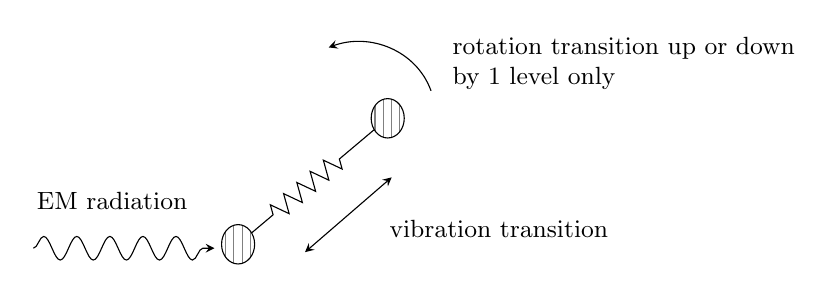
\begin{tikzpicture}[>=stealth, font=\small]
		\tikzset{atom/.style={draw, ellipse, minimum width=0.42cm, minimum height=0.5cm, inner sep=0pt, pattern=vertical lines, pattern color=gray}}
		\node[atom] (A) at (0,0) {};
		\node[atom] (B) at (1.9,1.6) {};
		\draw[decorate, decoration={zigzag, amplitude=0.12cm, segment length=0.22cm, pre length=0.35cm, post length=0.5cm}] (A) -- (B);
		\draw[->, decorate, decoration={snake, amplitude=0.15cm, segment length=0.42cm, post length=0.12cm}] (-2.6,-0.05) -- (-0.3,-0.05);
		\node at (-1.6,0.55) {EM radiation};
		\draw[<->] (0.85,-0.1) -- (1.95,0.85);
		\node[anchor=west] at (1.8,0.2) {vibration transition};
		\draw[->] (2.45,1.95) to[out=110, in=20] (1.15,2.5);
		\node[anchor=west, align=left] at (2.6,2.3) {rotation transition up or down\\by 1 level only};
	\end{tikzpicture}
	\caption{A vibration transition driven by EM radiation, accompanied by a rotation transition of one level.}
	\label{f:vibrot}
\end{figure}
% NOTE: the caption is added.

	\item[--] Since each vibration level can be associated w/ several rotation (sub-)levels, there are many possible vibration transitions within a population
	% NOTE: checked against Liou 2002, p. 17 ("the vibrational-rotational band in the intermediate infrared spectrum")
	% and p. 20 and Fig. 1.10b (p. 19): the rotational level spacings are smaller in the upper vibrational level, so the
	% line spacing decreases toward higher wavenumber (Lecture 10).
	\item[--] All vibration transitions require slightly different energy levels, which results in a series of closely spaced absorption lines that converge at short wavelength (i.e., higher freq) $\Rightarrow$ absorption bands in the intermediate infrared spectrum
	% NOTE: the handwritten U_v = hbar omega_k (nu_k + 1/2) is Liou 2002, Eq. 1.3.7 (p. 18), E_v = h nu~_k (upsilon_k + 1/2),
	% with hbar omega = h nu~. The vibrational quantum number (handwritten nu_k, Liou's upsilon_k) is written n_vib,k
	% (D99) and the mode's natural angular frequency omega_vib,k (D96); the mode index k (as in Liou) is flagged as D106.
	\item[--] Details are well beyond scope of the course, and we will simply state that the energy levels for vibrations is
	\begin{equation}
		\label{e:Ev}
		\mathcal{E}_\mathrm{v} = \hbar\omega_{\mathrm{vib},k}\left(n_{\mathrm{vib},k} + \tfrac{1}{2}\right),
	\end{equation}
	where $n_{\mathrm{vib},k} \equiv$ (integer) vibrational quantum number for $k$ normal mode\\
	(normal mode: components of system moving sinusoidally w/ same freq and relative phase)
	% NOTE: checked against Liou 2002, p. 18 ("fundamentals"; for triatomic molecules three normal modes; for linear
	% triatomic molecules the two bending modes are degenerate) and Fig. 3.3 (p. 71).
	\item[--] Different types of molecules have different normal modes, sometimes called fundamentals
	% NOTE: the handwritten percentages are fractions by volume (U&L 2014, p. 331 and Liou 2002, p. 71: O2 is 21% of air
	% by volume). Outside source (U.S. Standard Atmosphere): N2 78.08%, O2 20.95%, Ar 0.93%, CO2 ~0.04% (~420 ppmv today).
	\item[--] To illustrate, consider composition of Earth's atmosphere
	\begin{align*}
		&\mathrm{N_2} \sim 78.1\%\\
		&\mathrm{O_2} \sim 20.9\%\\
		&\mathrm{Ar} \sim 0.9\%\\
		&\mathrm{CO_2} \sim 0.04\%\\
		&\text{other } (\mathrm{H_2}, \mathrm{Ne}, \mathrm{He}, \mathrm{CH_4}, \ldots)
	\end{align*}
	% NOTE: added "(Figure~\ref{f:modes})".
	Vibrational normal modes (Figure~\ref{f:modes})
\end{itemize}

\begin{figure}[!htbp]
	\centering
	% Reproduces the handwritten table (page L4), element by element. Column heads "nu_1 symmetric", "nu_2 bending",
	% "nu_3 antisymmetric"; row heads "diatomic N2, O2, CO", "linear triatomic CO2, N2O", "bent (isosceles) triatomic".
	% Diatomic: nu_1 two atoms joined by a spring, outward arrows at both ends; nu_2, nu_3 "N/A". Linear triatomic: nu_1
	% three atoms joined by two springs, outward arrows at both ends; nu_2 three atoms with an upward arrow on the center
	% atom and downward arrows below the two end atoms, "and", then a second row with crossed circles (into the page) at
	% the ends and a dotted circle (out of the page) at the center, with a right brace labeled "same energy, different
	% quantum numbers"; nu_3 three atoms with arrows above them: left atom leftward, center atom rightward, right atom
	% leftward. Bent triatomic: nu_1 apex atom arrow up, left atom arrow down-left, right atom arrow down; nu_2 apex arrow
	% up, left atom arrow down-right, right atom arrow down-left (toward each other); nu_3 apex arrow right, left atom arrow
	% down-left, right atom arrow up-left (arrowhead at the atom, drawn from below).
	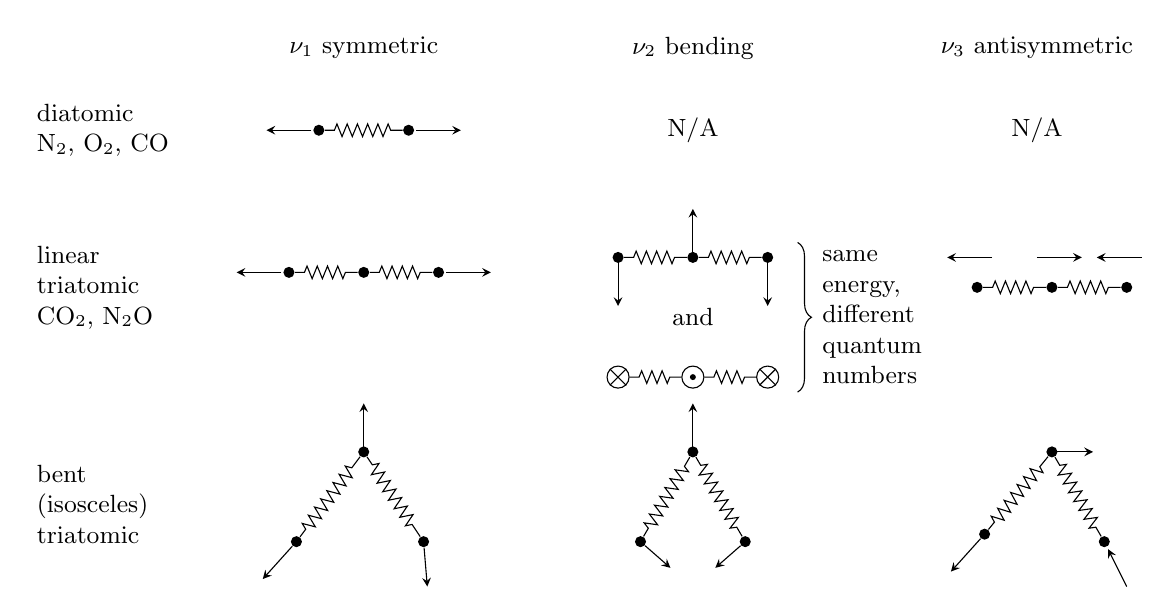
\begin{tikzpicture}[>=stealth, font=\small, scale=0.95]
		\tikzset{a/.style={circle, fill, inner sep=0pt, minimum size=4pt}}
		\tikzset{sp/.style={decorate, decoration={zigzag, amplitude=0.08cm, segment length=0.13cm, pre length=0.12cm, post length=0.12cm}}}
		% column heads
		\node at (4.0,6.6) {$\nu_1$ symmetric};
		\node at (8.4,6.6) {$\nu_2$ bending};
		\node at (13.0,6.6) {$\nu_3$ antisymmetric};
		% row heads
		\node[align=left, anchor=west] at (-0.5,5.5) {diatomic\\N$_2$, O$_2$, CO};
		\node[align=left, anchor=west] at (-0.5,3.4) {linear\\triatomic\\CO$_2$, N$_2$O};
		\node[align=left, anchor=west] at (-0.5,0.5) {bent\\(isosceles)\\triatomic};
		% diatomic
		\node[a] (d1) at (3.4,5.5) {}; \node[a] (d2) at (4.6,5.5) {};
		\draw[sp] (d1) -- (d2);
		\draw[->] (3.3,5.5) -- (2.7,5.5);
		\draw[->] (4.7,5.5) -- (5.3,5.5);
		\node at (8.4,5.5) {N/A};
		\node at (13.0,5.5) {N/A};
		% linear triatomic nu_1
		\node[a] (l1) at (3.0,3.6) {}; \node[a] (l2) at (4.0,3.6) {}; \node[a] (l3) at (5.0,3.6) {};
		\draw[sp] (l1) -- (l2); \draw[sp] (l2) -- (l3);
		\draw[->] (2.9,3.6) -- (2.3,3.6);
		\draw[->] (5.1,3.6) -- (5.7,3.6);
		% linear triatomic nu_2
		\node[a] (m1) at (7.4,3.8) {}; \node[a] (m2) at (8.4,3.8) {}; \node[a] (m3) at (9.4,3.8) {};
		\draw[sp] (m1) -- (m2); \draw[sp] (m2) -- (m3);
		\draw[->] (8.4,3.8) -- (8.4,4.45);
		\draw[->] (7.4,3.8) -- (7.4,3.15);
		\draw[->] (9.4,3.8) -- (9.4,3.15);
		\node at (8.4,3.0) {and};
		\node[draw, circle, inner sep=0pt, minimum size=0.28cm] (n1) at (7.4,2.2) {}; \draw (n1.north west) -- (n1.south east) (n1.north east) -- (n1.south west);
		\node[draw, circle, inner sep=0pt, minimum size=0.28cm] (n2) at (8.4,2.2) {}; \fill (8.4,2.2) circle (0.04);
		\node[draw, circle, inner sep=0pt, minimum size=0.28cm] (n3) at (9.4,2.2) {}; \draw (n3.north west) -- (n3.south east) (n3.north east) -- (n3.south west);
		\draw[sp] (n1) -- (n2); \draw[sp] (n2) -- (n3);
		\draw[decorate, decoration={brace, amplitude=5pt}] (9.8,4.0) -- (9.8,2.0);
		\node[align=left, anchor=west] at (10.0,3.0) {same\\energy,\\different\\quantum\\numbers};
		% linear triatomic nu_3
		\node[a] (r1) at (12.2,3.4) {}; \node[a] (r2) at (13.2,3.4) {}; \node[a] (r3) at (14.2,3.4) {};
		\draw[sp] (r1) -- (r2); \draw[sp] (r2) -- (r3);
		\draw[->] (12.4,3.8) -- (11.8,3.8);
		\draw[->] (13.0,3.8) -- (13.6,3.8);
		\draw[->] (14.4,3.8) -- (13.8,3.8);
		% bent nu_1
		\node[a] (b1t) at (4.0,1.2) {}; \node[a] (b1l) at (3.1,0.0) {}; \node[a] (b1r) at (4.8,0.0) {};
		\draw[sp] (b1l) -- (b1t); \draw[sp] (b1t) -- (b1r);
		\draw[->] (4.0,1.2) -- (4.0,1.85);
		\draw[->] (b1l) -- (2.65,-0.5);
		\draw[->] (b1r) -- (4.85,-0.6);
		% bent nu_2
		\node[a] (b2t) at (8.4,1.2) {}; \node[a] (b2l) at (7.7,0.0) {}; \node[a] (b2r) at (9.1,0.0) {};
		\draw[sp] (b2l) -- (b2t); \draw[sp] (b2t) -- (b2r);
		\draw[->] (8.4,1.2) -- (8.4,1.85);
		\draw[->] (b2l) -- (8.1,-0.35);
		\draw[->] (b2r) -- (8.7,-0.35);
		% bent nu_3
		\node[a] (b3t) at (13.2,1.2) {}; \node[a] (b3l) at (12.3,0.1) {}; \node[a] (b3r) at (13.9,0.0) {};
		\draw[sp] (b3l) -- (b3t); \draw[sp] (b3t) -- (b3r);
		\draw[->] (13.2,1.2) -- (13.75,1.2);
		\draw[->] (b3l) -- (11.85,-0.4);
		\draw[->] (14.2,-0.6) -- (13.95,-0.1);
	\end{tikzpicture}
	\caption{Vibrational normal modes of diatomic, linear triatomic, and bent triatomic molecules (after Liou 2002, Fig.~3.3). Crossed circles move into the page and the dotted circle out of it.}
	\label{f:modes}
\end{figure}
% NOTE: the caption is added. The handwritten "(see slides for movie of [curved arrow] for H2O)" is read as a pointer
% to the bent-triatomic row (low confidence); the Lecture 11 deck, slide 5, shows the vibrational (normal) modes of H2O.

\noindent(see slides for movie of these for H$_2$O)

%%%%%%%%%%%%%%%%%%%%%%%%%%%%%%%%%%%%%
% NOTE: subsection heading added; it is the handwritten bullet "Electronic energy U_e" (page L5).
\subsection{Electronic energy $\mathcal{E}_\mathrm{e}$}
\label{s:el}

\begin{itemize}
	\item[--] Represents electron energy levels within molecules
	% NOTE: the handwritten Delta E is written Delta script E, the difference of the molecular internal energies of
	% Eq. (e:E) (D95); master table D100 (formerly F8). Checked against U&L 2014, Eq. 8.10 (p. 329), f_0 = (E_m - E_l)/h,
	% and Liou 2002, Eq. 1.3.1 (p. 14); hbar omega = h f.
	\item[--] Moving from one energy level to another requires absorbing or emitting a specific frequency of EM radiation
	\begin{equation}
		\label{e:bohr}
		\Delta\mathcal{E} = \hbar\omega \qquad \text{(Bohr's formula)}
	\end{equation}
	\item[--] Bohr postulated the quantum theory based on the observed hydrogen spectrum and by building on Planck's oscillator concept
	\begin{itemize}
		% NOTE: checked against Liou 2002, Eq. 1.3.2 (p. 15), L = n(h/2 pi). The principal quantum number n is flagged
		% against the refractive index n (used in Sec. 2 of this lecture), D101; L against the Lorenz number, D102.
		\item[$\hookrightarrow$] Bohr postulated that the angular momentum $L$ of an electron could only take discrete values
		\begin{equation}
			\label{e:L}
			L = n_\mathrm{el}\hbar, \qquad n_\mathrm{el} \equiv \text{principal quantum number}
		\end{equation}
		% NOTE: scope added: "(for the hydrogen atom)"; Bohr's result is for a one-electron atom (Liou 2002, p. 15).
		\item[$\hookrightarrow$] From this selection rule, Bohr showed (for the hydrogen atom)
		\begin{equation}
			\label{e:Eesim}
			\mathcal{E}_\mathrm{e} \sim \frac{1}{n_\mathrm{el}^2}, \qquad n_\mathrm{el} = 1, 2, 3, \ldots
		\end{equation}
		where the constant of proportionality is a universal constant
		% NOTE: handwritten reads -m_e e^4/(8 eps_0 h^2 n^2); corrected to eps_0^2 because the energy requires it
		% dimensionally and Liou 2002, Eq. 1.3.3 (p. 15) has 8 eps_0^2 h^2. python3: m_e e^4/(8 eps_0^2 h^2) = 13.60 eV
		% = R_H h c with R_H = 1.097e7 m^-1 (Liou: 1.097e5 cm^-1). "e = charge of electron" is its magnitude, the
		% elementary charge (master table).
		\begin{equation}
			\label{e:Ee}
			\mathcal{E}_\mathrm{e} = -\frac{m_\mathrm{e}e^4}{8\varepsilon_0^2h^2n_\mathrm{el}^2} = -\frac{R_Hhc}{n_\mathrm{el}^2},
		\end{equation}
		\begin{itemize}
			\item[] $m_\mathrm{e} \equiv$ mass of electron,
			\item[] $e \equiv$ charge of electron,
			\item[] $h = 2\pi\hbar$,
			\item[] $\varepsilon_0 \equiv$ permittivity of free space,
			\item[] $R_H \equiv$ Rydberg constant for hydrogen.
		\end{itemize}
	\end{itemize}
\end{itemize}

%%%%%%%%%%%%%%%%%%%%%%%%%%%%%%%%%%%%%
% NOTE: subsection heading added; it is the handwritten bullet "Putting it all together" (page L6).
\subsection{Putting it all together}
\label{s:together}

(See Liou ``An Introduction to Atmospheric Radiation'' Ch.~1--3 for more details)

\begin{itemize}
	% NOTE: checked against Liou 2002, p. 71 (electronic energy is closely related to vibrational energy because both
	% derive from the elastic valence bonds; the force depends on the distance between the nuclei and their electronic
	% configuration).
	\item[--] Electronic and vibrational energy are closely related because both come from valence bonds that bind atoms into molecules
	\item[--] Sign and magnitude of force between two atoms in a molecule depends on 2 factors:
	\begin{itemize}
		\item distance between nuclei
		\item electron energy level
	\end{itemize}
	% NOTE: added "(Figure~\ref{f:pot})".
	\item[--] To illustrate, let us consider a simple potential energy curve for two electronic states and multiple possible vibration levels of a diatomic molecule (Figure~\ref{f:pot})
\end{itemize}

\begin{figure}[!htbp]
	\centering
	% Reproduces the handwritten sketch (page L6), element by element: axes "Energy" (arrowhead up) and "Distance between
	% nuclei" (arrowhead right); a ground-state curve with a tall repulsive wall at the left, its minimum near the bottom
	% and a plateau to the right, with three horizontal vibration levels labeled (handwritten nu_0, nu_1, nu_2, written
	% n_vib = 0, 1, 2, D99); an excited-state curve above it, shifted to larger distance, with three levels; a dashed
	% dissociation level decreasing from the upper left toward the excited-state plateau, with a squiggle leader to its
	% label; two upward arrows from the lowest ground level: T_1 (straight up through the excited well to above the
	% dissociation level) and T_2 (to the lowest
	% excited level), written script T_1, T_2 (D105); labels with leader lines: "repulsive forces pushing atoms apart
	% (like charges of nuclei repel)" to the left wall, "horizontal lines are vibration levels" to the excited levels,
	% "possible transitions due to absorption of photon" with arrows to T_1 and T_2, "Excited state (one possibility)",
	% "Ground state (minimum energy state)", and "Coulomb forces holding molecule together" with an arrow to the ground
	% curve's right branch. Curves are Morse potentials (after Liou 2002, Fig. 3.4).
	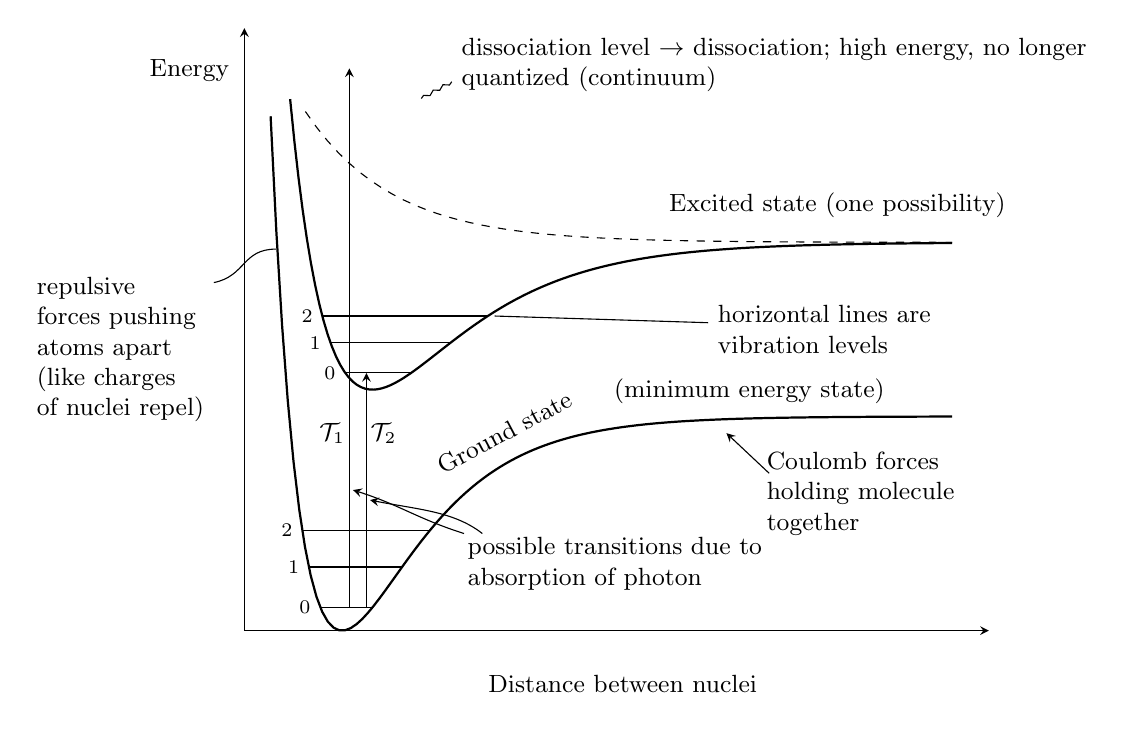
\begin{tikzpicture}[>=stealth, font=\small, xscale=1.55, yscale=0.85]
		% axes
		\draw[->] (0.8,0) -- (0.8,9.0) node[left, xshift=-2pt, pos=0.93] {Energy};
		\draw[->] (0.8,0) -- (6.9,0);
		\node at (3.9,-0.8) {Distance between nuclei};
		% ground state: V = 3.2 (1 - exp(-1.6 (r - 1.6)))^2
		\draw[thick, domain=1.015:6.6, samples=120] plot (\x, {3.2*(1-exp(-1.6*(\x-1.6)))^2});
		% excited state: V = 3.6 + 2.2 (1 - exp(-1.3 (r - 1.85)))^2
		\draw[thick, domain=1.175:6.6, samples=160] plot (\x, {3.6+2.2*(1-exp(-1.3*(\x-1.85)))^2});
		% dissociation level
		\draw[dashed, domain=1.3:6.6, samples=60] plot (\x, {5.8+1.7*exp(-1.4*(\x-1.4))});
		% vibration levels (between the Morse turning points)
		\foreach \E/\ra/\rb/\lab in {0.35/1.421/1.851/0, 0.95/1.328/2.092/1, 1.5/1.274/2.321/2} {
			\draw (\ra,\E) -- (\rb,\E);
			\node[font=\scriptsize, anchor=east] at (\ra,\E) {$\lab$};
		}
		\foreach \E/\ra/\rb/\lab in {0.25/1.627/2.166/0, 0.7/1.506/2.489/1, 1.1/1.439/2.795/2} {
			\draw (\ra,{3.6+\E}) -- (\rb,{3.6+\E});
			\node[font=\scriptsize, anchor=east] at (\ra,{3.6+\E}) {$\lab$};
		}
		% transitions (vertical, as in the scan)
		\draw[->] (1.66,0.35) -- (1.66,8.4);
		\draw[->] (1.80,0.35) -- (1.80,3.85);
		\node at (1.52,2.95) {$\mathcal{T}_1$};
		\node at (1.94,2.95) {$\mathcal{T}_2$};
		% labels
		\node[align=left, anchor=east] at (0.55,4.2) {repulsive\\forces pushing\\atoms apart\\(like charges\\of nuclei repel)};
		\draw (0.55,5.2) to[out=20, in=180] (1.06,5.7);
		\draw[decorate, decoration={snake, amplitude=0.6pt, segment length=4pt}] (2.25,7.95) -- (2.5,8.2);
		\node[align=left, anchor=west] at (2.5,8.45) {dissociation level $\rightarrow$ dissociation; high energy, no longer\\quantized (continuum)};
		\node[anchor=west] at (4.2,6.35) {Excited state (one possibility)};
		\draw (2.85,4.7) -- (4.6,4.6);
		\node[align=left, anchor=west] at (4.6,4.5) {horizontal lines are\\vibration levels};
		\node[align=left, anchor=west] at (2.55,1.0) {possible transitions due to\\absorption of photon};
		\draw[->] (2.6,1.45) to[out=150, in=-30] (1.69,2.1);
		\draw[->] (2.75,1.45) to[out=125, in=-20] (1.83,1.95);
		\node[anchor=south, rotate=28] at (3.0,2.72) {Ground state};
		\node[anchor=south west] at (3.75,3.25) {(minimum energy state)};
		\draw[->] (5.1,2.35) -- (4.75,2.95);
		\node[align=left, anchor=west] at (5.0,2.05) {Coulomb forces\\holding molecule\\together};
	\end{tikzpicture}
	\caption{Illustrative potential energy curves for two electronic states of a diatomic molecule, with vibration levels (horizontal lines) and two possible transitions due to absorption of a photon (after Liou 2002, Fig.~3.4). Numbers label the vibrational quantum number $n_\mathrm{vib}$.}
	\label{f:pot}
\end{figure}
% NOTE: the caption is added. The label "dissociation level -> ionization; high energy, no longer quantized
% (continuum)": handwritten "-> ionization" corrected to "-> dissociation" (instructor decision, 2026-09-30): Liou 2002 distinguishes the dissociation
% potential (separation of the atoms) from the ionization potential (removal of an electron; p. 71) and calls the
% unquantized continuum above this level dissociation (p. 73: transition 1 leads to "a state that is not quantized,
% denoted by the dissociation level"); an unstable excited molecule may decompose into its atoms "and photoionization
% may also occur" (p. 72), which generally requires higher energy.

\begin{itemize}
	\item[--] Key points from potential curve
	\begin{enumerate}
		% NOTE: checked against Liou 2002, p. 72.
		\item Energy gain from ground state to excited state (due to electronic transition) is simply the difference in minimum potential energies
		\item Vibrations are represented as horizontal lines showing changes in distances between nuclei
		\begin{itemize}
			\item[$\hookrightarrow$] vibration transitions (always accompanied by rotation transitions) entail change in energy level $\Rightarrow$ range of oscillation
		\end{itemize}
		% NOTE: the handwritten transition labels T_1, T_2 are written script T_1, T_2 (T is temperature only, D19);
		% master table D105. Checked against Liou 2002, p. 73.
		\item Illustrated transitions $\mathcal{T}_1$ and $\mathcal{T}_2$
		\begin{itemize}
			\item $\mathcal{T}_1$ from ground state to dissociation, which is not quantized $\Rightarrow$ a continuum of absorption wavelengths near energy associated w/ $\mathcal{T}_1$
			\item $\mathcal{T}_2$ remains quantized $\Rightarrow$ transition to specific vibration level $\Rightarrow$ absorption spectrum will have discrete wavelengths in absence of disturbances
		\end{itemize}
		% NOTE: checked against Liou 2002, p. 73.
		\item At atmospheric temperatures, most molecules are in ground vibrational states $\Rightarrow$ transitions $\mathcal{T}_1$ and $\mathcal{T}_2$ are representative of transitions in atmosphere
		% NOTE: kept as handwritten; scope for the instructor: Liou 2002, p. 73, says "many absorption processes associated
		% with diatomic molecules are largely a combination of electronic and vibrational transitions that occur in the
		% UV, visible, and near IR"; at thermal-infrared and microwave frequencies atmospheric absorption is by
		% vibration-rotation and pure rotation transitions (U&L 2014, p. 329; Liou p. 17), with no electronic transition.
		\item Most absorption processes in atmosphere are a combination of electronic and vibrational transitions as depicted
		\begin{itemize}
			\item[$\hookrightarrow$] These generally occur in UV, visible, and near IR frequencies
		\end{itemize}
	\end{enumerate}
\end{itemize}

%%%%%%%%%%%%%%%%%%%%%%%%%%%%%%%%%%%%%
% NOTE: section heading added; it is the handwritten bullet "Effects of disturbances on absorption (and emission)
% spectrum" (page L8).
\section{Effects of disturbances on absorption (and emission) spectrum}
\label{s:broad}

\begin{itemize}
	% NOTE: checked against U&L 2014, p. 329 (Sec. 8-2.2) and Liou 2002, p. 21 (Sec. 1.3.2).
	\item[--] Previous discussion applicable to isolated, undisturbed, stationary molecular system
	\item[--] But molecules are in constant motion, interacting and colliding w/ one another and w/ other matter (e.g., dust particles)\\
	$\Rightarrow$ Energy levels during transitions change slightly due to external influences on molecules $\Rightarrow$ radiation emitted during repeated transitions is polychromatic (multiple frequencies), causing absorption spectra lines of finite width
	\item[--] Increased absorption width called ``line broadening''
	% NOTE: kept as handwritten. Liou 2002, p. 21, lists a third cause, natural broadening (loss of energy in emission),
	% "practically negligible as compared to that caused by collisions and the Doppler effect".
	\item[--] Two main causes of line broadening
	\begin{enumerate}
		\item Collision or pressure broadening, which is dominant in troposphere
		\item Doppler broadening -- results from different thermal velocities of atoms and molecules (Doppler effect) $\rightarrow$ only important in upper atmosphere where pressures are very low
	\end{enumerate}
	% NOTE: checked against U&L 2014, p. 329 (pressure broadening "is the most important for atmospheric absorption in
	% the microwave region") and Liou 2002, p. 21 (collision broadening prevails below about 20 km).
	\item[--] Pressure broadening is, in general, the dominant process influencing absorption and emission in Earth's atmosphere
\end{itemize}

%%%%%%%%%%%%%%%%%%%%%%%%%%%%%%%%%%%%%
% NOTE: subsection heading added (the handwriting's "Pressure broadening (cont.)" on page L11 names the topic).
\subsection{Pressure broadening}
\label{s:pressure}

\begin{itemize}
	% NOTE: "Lecture 1" refers to the damped harmonic oscillator of Lecture 1, Eq. (e:oscillator) there. The handwritten
	% gamma (damping coefficient) is written nu, as in Lecture 1 (master table D9: gamma is reserved for the propagation
	% constant).
	\item We can understand pressure broadening by going back to our discussion of permittivity in Lecture~1 where we modeled polarization of materials as a damped harmonic oscillator. Same model applies for pressure broadening.
	\item Therefore, dielectric constant is
	\begin{equation}
		\label{e:eps}
		\varepsilon(\omega) = 1 + \frac{\omega_p^2}{(\omega_0^2 - \omega^2) + j\nu\omega},
	\end{equation}
	where
	% NOTE (page L10): handwritten reads "omega_p = N e^2/(eps_0 m_e)"; corrected to omega_p^2, as in Lecture 1, because the
	% right side has units of s^-2 and Eq. (e:eps) requires the square (Lecture 1, Eq. e:oscillator; Liou 2002,
	% Eq. D.16a, p. 531, in Gaussian units 4 pi N e^2/m_e).
	\begin{itemize}
		\item[] $\omega_p \equiv$ plasma frequency, $\omega_p^2 = \dfrac{Ne^2}{\varepsilon_0m_\mathrm{e}}$,
		\item[] $e \equiv$ electron charge,
		% NOTE (page L10): handwritten reads "number of dipoles"; the dimensions of omega_p^2 require N to be a number
		% density (m^-3), as in Lecture 1 and the Variables table.
		\item[] $N \equiv$ number of dipoles per unit volume,
		\item[] $m_\mathrm{e} \equiv$ mass of electron,
		\item[] $\varepsilon_0 \equiv$ permittivity of free space,
		\item[] $\omega_0 \equiv$ natural frequency,
		\item[] $\nu \equiv$ damping coef.
	\end{itemize}
	% NOTE (page L10): handwritten reads kappa_a = 2 K_0 n'' = 2 K_0 Im{sqrt(eps)}; K_0 written k_0 (D14), and the sign of the second
	% form corrected: with e^{j omega t} and eps = eps' - j eps'', sqrt(eps) = n' - j n'', so Im{sqrt(eps)} = -n'' < 0
	% (master table and Lecture 9: kappa_a = -2 k_0 Im{sqrt(eps)} = 2 alpha; U&L 2014, Eqs. 8.12, 8.16a, 8.17, p. 330).
	% NOTE (page L10): handwritten reads kappa_a = S gamma/((omega - omega_0)^2 + gamma^2) with S = omega_p^2/c; corrected to the
	% form below because, with the gamma (= nu) of Eq. (e:eps), the half-width at half-maximum of the line in omega is
	% nu/2, not nu, and the strength is off by a factor 2. Derivation: near resonance (|omega - omega_0| << omega_0,
	% nu << omega_0) and for a dilute gas (|eps - 1| << 1), omega_0^2 - omega^2 ~ 2 omega_0 (omega_0 - omega) and
	% sqrt(eps) ~ 1 + (eps - 1)/2 give
	%   n'' = (omega_p^2/(4 omega_0)) (nu/2)/((omega - omega_0)^2 + (nu/2)^2),
	%   kappa_a = 2 (omega/c) n'' ~ (omega_p^2/(2c)) (nu/2)/((omega - omega_0)^2 + (nu/2)^2).
	% Written in the normalized Lorentz form of Liou 2002, Eq. 1.3.10 (p. 21) and Eq. D.18 (p. 531), with S the
	% integrated line strength (Liou Eq. 1.3.11): S = int kappa_a d omega = pi omega_p^2/(2c). (Liou, Eqs. D.17-D.18,
	% Gaussian units, with nu~ as ordinary frequency in App. D (Sec. 1.3 uses nu for wavenumber): half-width alpha_N = gamma/(4 pi), S = pi N e^2/(m_e c); converted to SI and omega
	% these give the same result.) python3: the exact kappa_a from Eq. (e:eps) agrees with this to 0.3% within three
	% half-widths of omega_0 for nu/omega_0 = 1e-4, and its integral over the line is S to 0.02%. The normalized form
	% also makes the comparison with the Doppler line in Figure (f:comp) consistent (same S).
	\item Defining the power absorption coef as we did for volume scattering, we have
	\begin{align}
		\kappa_\mathrm{a} &= 2k_0n'' = -2k_0\,\mathrm{Im}\{\sqrt{\varepsilon}\} \nonumber\\
		&= \frac{S}{\pi}\,\frac{\nu/2}{(\omega-\omega_0)^2 + (\nu/2)^2} \quad \rightarrow \text{sometimes called the Lorentz profile} \label{e:lorentz}
	\end{align}
	where $S = \dfrac{\pi\omega_p^2}{2c} \equiv$ spectral line strength (near resonance, for a dilute gas).
	% NOTE (page L10): a faint erasure residue precedes omega_p^2 in the handwritten numerator; not transcribed
	% (low confidence).
	% NOTE (page L10): handwritten reads n' = 1 + (omega_p^2/omega_0) (omega - omega_0)/((omega - omega_0)^2 + gamma^2); corrected to
	% the form below (sign, factor 1/4, and half-width nu/2) by the same derivation: n' - 1 = Re{eps - 1}/2 =
	% (omega_p^2/(4 omega_0)) (omega_0 - omega)/((omega - omega_0)^2 + (nu/2)^2). Liou 2002, Eq. D.17 (p. 531):
	% m_r - 1 = -(N e^2/(4 pi m_e nu~_0)) (nu~ - nu~_0)/((nu~ - nu~_0)^2 + alpha_N^2), the same in SI and omega. The
	% corrected sign agrees with the handwritten plot (n' > 1 below resonance, n' < 1 above) and with item 3 below.
	% python3 check as above (0.1%).
	\item Similarly, the real component of the index of refraction is
	\begin{equation}
		\label{e:nprime}
		n' = 1 - \frac{\omega_p^2}{4\omega_0}\,\frac{\omega - \omega_0}{(\omega-\omega_0)^2 + (\nu/2)^2}
	\end{equation}
	% NOTE: added "(Figure~\ref{f:disp})".
	\item[--] Plotting $\kappa_\mathrm{a}$ and $n'$ (Figure~\ref{f:disp})
\end{itemize}

\begin{figure}[!htbp]
	\centering
	% Reproduces the handwritten plot (page L11), element by element: horizontal axis with arrowheads at both ends,
	% ticks -3, -2, -1, 1, 2, 3, labeled (handwritten) 4 pi (omega - omega_0)/gamma; vertical axis with arrowheads at both
	% ends; solid curve n' - 1 (label "n' - 1" at its left), maximum at -1 and minimum at +1, with vertical dashed lines
	% from them to the axis; dotted curve kappa_a (label at its right tail). Annotations with leader lines: "'normal'
	% dispersion (dn'/domega > 0)" to the left branch; "peak kappa_a when omega = omega_0 => resonance" to the peak of
	% kappa_a; "n' = 1 when omega = omega_0" to the origin; "n' < 1 !!!" to the right branch; "'anomalous' dispersion
	% (dn'/domega < 0)" to the steep central section. Curves plotted from Eqs. (e:lorentz) and (e:nprime) in the
	% variable x = 2(omega - omega_0)/nu: kappa_a proportional to 1/(1 + x^2) and n' - 1 proportional to -x/(1 + x^2),
	% each scaled to a peak of 1 (arbitrary units).
	% NOTE (page L11): handwritten axis label 4 pi (omega - omega_0)/gamma corrected to 2(omega - omega_0)/nu, because the extrema of
	% n' and the half-maximum points of kappa_a are at omega - omega_0 = +-nu/2 (Eqs. e:lorentz, e:nprime; python3: exact
	% extrema of n' from Eq. (e:eps) at (omega - omega_0)/(nu/2) = -1.02, +0.98 for nu/omega_0 = 0.09). The handwritten
	% label is Liou's (nu~ - nu~_0)/alpha_N with alpha_N = gamma/(4 pi) (Liou 2002, Fig. D.1, p. 531), which holds for
	% the ordinary frequency f = omega/2 pi (App. D uses nu~ for ordinary frequency, whereas Sec. 1.3 uses nu
	% for wavenumber: a notation switch), not for omega: 4 pi (f - f_0)/nu = 2(omega - omega_0)/nu.
	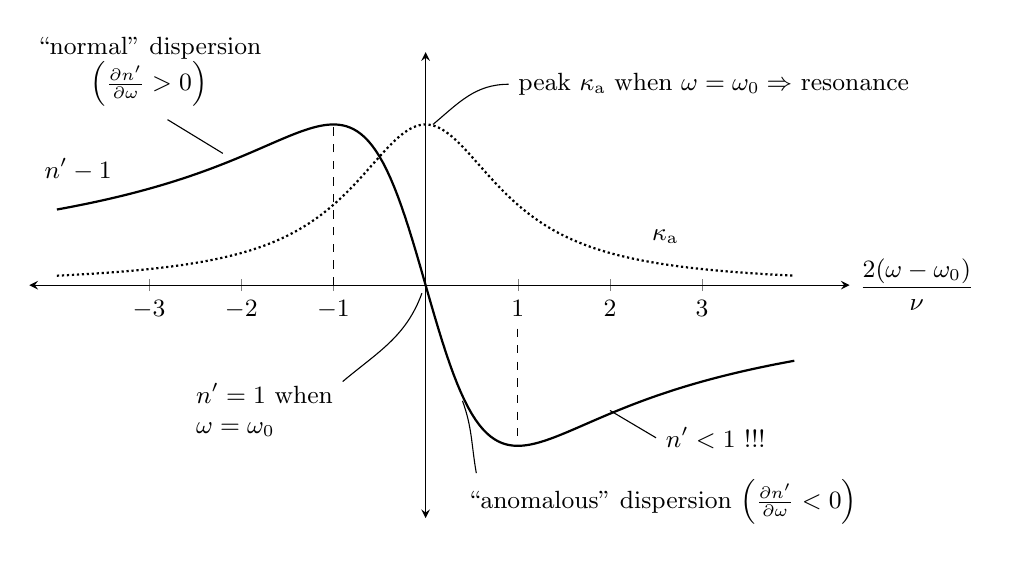
\begin{tikzpicture}[>=stealth, font=\small]
		\begin{axis}[width=12cm, height=7.5cm, axis lines=middle, axis line style={<->},
			xmin=-4.3, xmax=4.6, ymin=-1.45, ymax=1.45, xtick={-3,-2,-1,1,2,3}, ytick=\empty,
			xlabel={$\dfrac{2(\omega-\omega_0)}{\nu}$}, xlabel style={anchor=west, at={(axis cs:4.6,0)}},
			tick label style={font=\small}, xticklabel style={yshift=0pt}, clip=false]
			\addplot[thick, domain=-4:4, samples=200] {-2*x/(1+x^2)};
			\addplot[densely dotted, thick, domain=-4:4, samples=200] {1/(1+x^2)};
			\draw[dashed] (axis cs:-1,0) -- (axis cs:-1,1);
			\draw[dashed] (axis cs:1,-0.27) -- (axis cs:1,-1);
			\node[anchor=east] at (axis cs:-3.3,0.72) {$n'-1$};
			\node at (axis cs:2.6,0.3) {$\kappa_\mathrm{a}$};
			\node[align=center, anchor=south] at (axis cs:-3.0,1.05) {``normal'' dispersion\\$\left(\frac{\partial n'}{\partial\omega} > 0\right)$};
			\draw (axis cs:-2.8,1.03) -- (axis cs:-2.2,0.82);
			\node[anchor=west] at (axis cs:0.9,1.25) {peak $\kappa_\mathrm{a}$ when $\omega = \omega_0 \Rightarrow$ resonance};
			\draw (axis cs:0.9,1.25) to[out=180, in=40] (axis cs:0.08,1.0);
			\node[align=left, anchor=north east] at (axis cs:-0.9,-0.55) {$n' = 1$ when\\$\omega = \omega_0$};
			\draw (axis cs:-0.9,-0.6) to[out=40, in=-110] (axis cs:-0.04,-0.05);
			\node[anchor=west] at (axis cs:2.5,-0.95) {$n' < 1$ !!!};
			\draw (axis cs:2.5,-0.95) -- (axis cs:2.0,-0.78);
			\node[align=left, anchor=north west] at (axis cs:0.35,-1.15) {``anomalous'' dispersion $\left(\frac{\partial n'}{\partial\omega} < 0\right)$};
			\draw (axis cs:0.55,-1.17) to[out=100, in=-70] (axis cs:0.4,-0.72);
		\end{axis}
	\end{tikzpicture}
	\caption{Absorption coefficient $\kappa_\mathrm{a}$ (dotted) and real part of the index of refraction, $n'-1$ (solid), near a resonance at $\omega_0$ (arbitrary units).}
	\label{f:disp}
\end{figure}
% NOTE: the caption is added.

% NOTE: nesting follows the scan (pages L11-L13): "- Take-aways from kappa_a and n' plot" has two dot items, "For
% kappa_a" (page L11) and "For n'" (page L13). The dash item "- Since molecular collision plays a key role in damping"
% (page L12) is indented less than the dot items but more than "- Take-aways" and continues the damping take-away 2)
% for kappa_a, so it is set as a dash item inside "For kappa_a" (interpretive).
\begin{itemize}
	\item[--] Take-aways from $\kappa_\mathrm{a}$ and $n'$ plot:
	\begin{itemize}
		\item For $\kappa_\mathrm{a}$:
		\begin{enumerate}
			\item[1)] Peak absorption at resonance freq $\omega_0$
			% NOTE: the half-width at half-maximum is nu/2 (Eq. e:lorentz). The collision picture is Liou 2002, pp.
			% 22-23: collisions destroy the phase coherence of the emitted wave train.
			\item[2)] width of $\kappa_\mathrm{a}$ defined by damping coef $\nu$
			\begin{itemize}
				\item[$\rightarrow$] what causes damping? emission (no apparent dissipative mechanisms)\\
				But collisions play a role $\rightarrow$ collision of molecules causes phase shift in emitted EM wave. Collisions $\rightarrow$ random $\Rightarrow$ population of molecules emit EM waves w/ random phases $\Rightarrow$ reduced phase coherence $\Rightarrow$ damping
			\end{itemize}
		\end{enumerate}
		\begin{itemize}
			\item[--] Since molecular collision plays a key role in damping, we may suppose a relationship between damping coef and temperature and pressure
			% NOTE (page L12): checked against Liou 2002, Eq. 1.3.14 (p. 23), alpha = alpha_0 (p/p_0)(T_0/T)^n with n from
			% 1/2 to 1 and T_0 = 273 K, for the half-width alpha; the damping coefficient nu = 2 x (half-width in omega)
			% scales the same way. The handwritten exponent (Liou's n) is read as delta (low confidence; possibly g or 8);
			% master table D109. "T_0 = 273 K" is kept as handwritten (Liou's reference temperature); see the NOTE at
			% Eq. (e:nuz) and master table D116.
			\begin{equation}
				\label{e:nuPT}
				\nu = \nu_0\left(\frac{P}{P_0}\right)\left(\frac{T_0}{T}\right)^\delta \qquad \text{for } \tfrac{1}{2} \le \delta \le 1
			\end{equation}
			\begin{itemize}
				\item[] $\nu_0 \equiv$ reference damping coef ($\nu = \nu_0$ for $P = P_0$ and $T = T_0$),
				\item[] $P_0 \equiv$ atmospheric pressure at sea level,
				\item[] $T_0 = 273$~K.
			\end{itemize}
			% NOTE (page L12): checked by derivation: with P = P_0 exp(-z/H_p) (Lecture 10, Eq. e:Hp) and T = T_0 - a z
			% (Lecture 10), T_0/T = (1 - a z/T_0)^-1, so (T_0/T)^delta = (1 - a z/T_0)^-delta. "note sign" refers to the
			% handwritten minus sign on the exponent.
			% NOTE (page L12): kept as handwritten, but in (1 - a z/T_0) T_0 is the Lecture 10 sea-level standard
			% temperature (288.15 K; U&L 2014, Eq. 8.1, p. 327), whereas Eq. (e:nuPT) defines T_0 = 273 K (the reference
			% temperature of nu_0), so the reference and surface temperatures are conflated (master table D116). The
			% effect is small: python3 at z = 12 km, H_p = 8.4 km, a = 6.5 K/km, delta = 1/2: nu/nu_0 = 0.281 with
			% T_0 = 288.15 K in Eq. (e:nuz) vs 0.284 with T_0 = 273 K (~1%); keeping the reference at 273 K and the
			% surface at 288.15 K, (273/(288.15 K - a z))^delta e^{-z/H_p} = 0.273 (~3%). For delta = 1: 0.329, 0.336,
			% 0.311.
			Plugging in temperature lapse rate for troposphere and $P$ profile (see last lecture)
			\begin{equation}
				\label{e:nuz}
				\frac{\nu}{\nu_0} = e^{-z/H_p}\left(1 - \frac{az}{T_0}\right)^{-\delta} \quad \text{(note sign)}
			\end{equation}
			\begin{itemize}
				\item[] $H_p \simeq 8.4$~km,
				\item[] $a \simeq 6.5$~K/km.
			\end{itemize}
			% NOTE (page L12): kept as handwritten. python3 with Eq. (e:nuz), H_p = 8.4 km, a = 6.5 K/km, z = 12 km:
			% nu/nu_0 = 0.27-0.34 over delta = 1/2 to 1 and the three T_0 treatments above, i.e., a decrease by a factor
			% ~3 (1/e = 0.37); with the exact standard-atmosphere pressure at 12 km (0.19 P_0), 0.22-0.25.
			% NOTE: handwritten reads "decreases by roughly 1/e"; changed to "to" because Eq. (e:nuz) gives nu/nu_0 ~ 0.28-0.34
			% at 12 km (instructor decision 2026-09-30).
			$\Rightarrow$ $\nu$ decreases to roughly $1/e$ of its surface value from surface to tropopause (${\sim}12$~km altitude)
		\end{itemize}
		\item For $n'$:
		\begin{enumerate}
			% NOTE (page L13): handwritten v_p = omega/(K_0 n') = c/n' is written u_p = omega/(k_0 n') (D15, D14).
			\item For most $\omega$, $\dfrac{\partial n'}{\partial\omega} > 0 \rightarrow$ ``normal'' dispersion\\
			(recall phase velocity $u_p = \dfrac{\omega}{k_0n'} = \dfrac{c}{n'}$)\\
			but near resonance freq $\omega_0$, $\dfrac{\partial n'}{\partial\omega} < 0$\\
			$\rightarrow$ ``anomalous'' dispersion $\rightarrow$ only occurs where $\kappa_\mathrm{a}$ is large\\
			and
			% NOTE (page L13): handwritten reads "dn'/domega = 0 when omega = omega_0 + gamma/(4 pi)"; corrected to
			% omega_0 +- nu/2 because, from Eq. (e:nprime), n' has a maximum at omega_0 - nu/2 and a minimum at
			% omega_0 + nu/2 (derivation; python3 on the exact Eq. e:eps: -1.02 and +0.98 half-widths). The handwritten
			% gamma/(4 pi) is Liou's half-width alpha_N in ordinary frequency (Liou 2002, App. D, p. 531, where nu~
			% denotes ordinary frequency), i.e., nu/2 in omega; see the NOTE at Figure (f:disp). Both boundaries of the
			% anomalous region are given (the handwriting gives the upper one).
			\begin{equation}
				\label{e:dndw}
				\frac{\partial n'}{\partial\omega} = 0 \quad \text{when } \omega = \omega_0 \pm \frac{\nu}{2}
			\end{equation}
			% NOTE (page L13): handwritten reads "omega = omega_n"; corrected to omega_0 (the resonance; cf. the plot,
			% "n' = 1 when omega = omega_0", and Eq. e:nprime).
			\item $n' = 1$ when $\omega = \omega_0$
			\item Strikingly, $n' < 1$ when $\omega > \omega_0$ (in vicinity of $\omega_0$, not in general)\\
			This implies $u_p > c$ !!! called ``superluminal'' $\rightarrow$ many of you noticed this in question~1 of pset~1\\
			Is it physical? Yes\\
			Explanation:
			\begin{itemize}
				\item $n'$ varies w/ $\omega$ $\Rightarrow$ atmosphere is dispersive, at least in the neighborhood of $\omega_0$
				\item Phase velocity only tells us how fast a wave of a given frequency travels (i.e., how fast a plane of constant phase travels)
				\item In a dispersive material, waves of different frequencies travel at different speeds $\Rightarrow$ wave packet distorts (Figure~\ref{f:packet})
			\end{itemize}
		\end{enumerate}
	\end{itemize}
\end{itemize}
% NOTE: added "(Figure~\ref{f:packet})" above.

\begin{figure}[!htbp]
	\centering
	% Reproduces the handwritten sketch (page L14): a distorted wave packet, a small oscillation at the left, the largest
	% excursions near the center, and decaying, irregular oscillations to the right, about 3.5 cycles in all and no long
	% flat tails (no axes). Drawn as a Gaussian
	% envelope times a chirped cosine.
	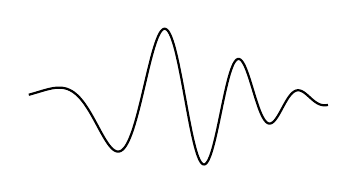
\begin{tikzpicture}
		\begin{axis}[width=5.5cm, height=3.6cm, axis lines=none, xmin=-1.5, xmax=1.8, ymin=-1.1, ymax=1.1]
			\addplot[thick, domain=-1.45:1.75, samples=400] {exp(-((x+0.05)/1.0)^2)*cos(deg(6.6*x+1.4*x^2))*(1+0.25*x)};
		\end{axis}
	\end{tikzpicture}
	\caption{A wave packet distorts as it propagates through a dispersive material.}
	\label{f:packet}
\end{figure}
% NOTE: the caption is added.

\begin{itemize}
	% NOTE: handwritten v_g = dw/dK is written u_g = domega/dk (u_p pattern, D15; D14); master table D115.
	\item Useful then to define the rate of propagation of a plane of constant amplitude
	\begin{equation}
		\label{e:ug}
		\rightarrow \text{group velocity } u_g = \frac{\partial\omega}{\partial k}
	\end{equation}
	% NOTE: k is the wavenumber in the medium, omega/u_p = k_0 n' (instructor decision 2026-09-30, master table D163);
	% with k = omega/c the definition would give u_g = c identically.
	where $k = \omega/u_p = k_0n'$ is the wavenumber in the medium ($k_0 = \omega/c$ in free space)
	% NOTE: kept, with the scope added in parentheses. Outside source (Jackson 1999, Classical Electrodynamics, 3rd ed.,
	% Sec. 7.8-7.11; Brillouin 1960): the group velocity is the velocity of energy and information only where absorption
	% is weak (away from the line center); in the anomalous-dispersion region of an absorption line u_g itself can exceed c
	% or become negative, and the signal front never travels faster than c.
	\item Energy (information) travels at the group velocity (where absorption is weak, i.e., away from line centers) $\Rightarrow$ no requirement that $u_p \le c$ even though $u_p < c$ is by far the most common situation\\
	(most of you will never encounter a case where $u_p > c$ but this example is useful to highlight $u_g = \partial\omega/\partial k$, an extremely useful concept that some of you will encounter in practice)
\end{itemize}

%%%%%%%%%%%%%%%%%%%%%%%%%%%%%%%%%%%%%
% NOTE: subsection heading added; it is the handwritten bullet "Doppler broadening" (page L15).
\subsection{Doppler broadening}
\label{s:doppler}

\begin{itemize}
	% NOTE: kept, with the scope added in parentheses. Liou 2002, p. 24: from about 20 to 50 km, line shapes are
	% determined by both collision and Doppler broadening (Voigt profile), and p. 21: "in the upper atmosphere, we find a
	% combination of collision and Doppler broadenings". The Doppler width is proportional to the line frequency (Liou
	% Eq. 1.3.18), so microwave lines stay pressure-broadened to higher altitudes. python3: Doppler half-width (HWHM,
	% alpha_D sqrt(ln 2)) at 230 K is 0.058 MHz for the 60 GHz O2 lines and 16 MHz for the 15-um CO2 band, while the
	% pressure half-widths at 1013 mb are ~300-3000 MHz (Liou p. 23: alpha_0 = 0.01-0.1 cm^-1), so the two are equal
	% near P/P_0 ~ 1e-2 for IR lines (~30 km) and ~2e-4 to 2e-5 for microwave lines (~65-80 km).
	\item[--] Pressure broadening is the dominant process in much of the atmosphere, but in the upper atmosphere (stratosphere and beyond) pressures are low $\rightarrow$ pressures decrease w/ altitude while temperature increases w/ altitude $\Rightarrow$ damping due to pressure broadening decreases rapidly w/ altitude\\
	% NOTE: handwritten reads "in stratosphere and above, pressure broadening is negligible and Doppler broadening becomes
	% dominant"; scoped because the Doppler and pressure widths are equal near ~30 km for IR lines and ~65-80 km for
	% microwave lines (see NOTE above; Liou 2002, pp. 21, 24).
	$\Rightarrow$ with increasing altitude through the stratosphere and above, Doppler broadening becomes increasingly important and eventually dominant (for infrared lines, both matter from about 20 to 50~km; microwave lines remain pressure broadened to higher altitudes)
	% NOTE: checked against Liou 2002, Eqs. 1.3.17-1.3.18 (p. 24), k_nu = S/(alpha_D sqrt(pi)) exp[-((nu - nu_0)/alpha_D)^2],
	% alpha_D = nu_0 (2KT/mc^2)^(1/2), with Liou's wavenumber nu (cycles per length) = k/(2 pi) for the angular
	% wavenumber k_0 used here (free space, D163); K, K_0, K_B are written k, k_0, k_B (D14). With this normalization S is the integral of
	% kappa_d over k/(2 pi), whereas S in Eq. (e:lorentz) is the integral over omega (= 2 pi c times the integral over
	% k/(2 pi)); the comparison in Figure (f:comp) uses the same S in the same variable. Here k_0 = omega_0/c is the
	% wavenumber at the line center, written k_line (master table D113); kappa_{a,D} (D111), alpha_D (D112), m_m (D114).
	\item[--] From the kinetic theory of gases and assuming thermodynamic equilibrium, it can be shown that the absorption coef for Doppler broadening is
	\begin{equation}
		\label{e:doppler}
		\kappa_{\mathrm{a},\mathrm{D}} = \frac{S}{\alpha_\mathrm{D}\sqrt{\pi}}\exp\left\{-\left(\frac{k_0-k_\mathrm{line}}{2\pi\alpha_\mathrm{D}}\right)^2\right\}
	\end{equation}
	where
	\begin{equation}
		\label{e:alphaD}
		\alpha_\mathrm{D} = \frac{k_\mathrm{line}}{2\pi}\sqrt{\frac{2k_BT}{m_\mathrm{m}c^2}},
	\end{equation}
	\begin{itemize}
		\item[] $k_B \equiv$ Boltzmann's constant,
		\item[] $m_\mathrm{m} \equiv$ molecular mass.
	\end{itemize}
	% NOTE: added (instructor decision on master table D110, 2026-09-30).
	Here the line strength $S$ is the integral of the absorption coefficient over $k/2\pi$; in Eq.~\eqref{e:lorentz} it is the integral over $\omega$, so the two differ by the factor $2\pi c$.
\end{itemize}

%%%%%%%%%%%%%%%%%%%%%%%%%%%%%%%%%%%%%
\subsection{Comparing pressure and Doppler broadening}
\label{s:compare}

\begin{figure}[H]
	\centering
	% Reproduces the handwritten plot (page L16), element by element: vertical axis (arrowhead up) labeled "kappa_a,
	% kappa_d"; horizontal axis (arrowhead right) with ticks -3, -2, 0, 2, 3, labeled (handwritten) (K - K_0)/alpha; a
	% dashed curve kappa_d, taller and narrower, near zero beyond +-2; a solid curve kappa_a, lower, with long tails
	% still above the axis at +-3. Curves plotted with the same S and the same width parameter, as in Liou 2002, Fig. 1.11
	% (p. 22): Lorentz (1/pi)/(1 + x^2) and Doppler exp(-x^2)/sqrt(pi) in x = (k - k_0)/(2 pi alpha).
	% NOTE: handwritten axis label (K - K_0)/alpha and "alpha = gamma/(4 pi)" for pressure broadening; corrected to
	% (k - k_0)/(2 pi alpha) and alpha = nu/(4 pi c) because (i) in Eq. (e:doppler) the Gaussian's width parameter in k is
	% 2 pi alpha_D (Liou's variable is k/(2 pi)), so on the handwritten axis the Doppler curve would reach e^-1 only at
	% 2 pi ~ 6.3 rather than near 1 as sketched; (ii) the Lorentz half-width nu/2 in omega (Eq. e:lorentz) is nu/(2c) in
	% k = omega/c and nu/(4 pi c) in k/(2 pi), in the same units (1/m) as alpha_D; the handwritten gamma/(4 pi) is the
	% half-width in ordinary frequency (Liou App. D, alpha_N = gamma/(4 pi)), in s^-1. Derivation.
	\begin{tikzpicture}[>=stealth, font=\small]
		\begin{axis}[width=11cm, height=5.4cm, axis lines=middle, axis line style={->},
			xmin=-3.6, xmax=4.0, ymin=0, ymax=0.68, xtick={-3,-2,2,3}, extra x ticks={0}, extra x tick style={tick label style={xshift=-5pt}}, ytick=\empty,
			xlabel={$\dfrac{k_0-k_\mathrm{line}}{2\pi\alpha}$}, xlabel style={anchor=west, at={(axis cs:4.0,0)}},
			clip=false]
			\addplot[thick, domain=-3.5:3.5, samples=200] {1/(pi*(1+x^2))};
			\addplot[thick, dashed, domain=-2.6:2.6, samples=200] {exp(-x^2)/sqrt(pi)};
			\node[anchor=west] at (axis cs:0.08,0.66) {$\kappa_\mathrm{a}, \kappa_{\mathrm{a},\mathrm{D}}$};
			\node[anchor=west] at (axis cs:0.75,0.47) {$\kappa_{\mathrm{a},\mathrm{D}}$};
			\node[anchor=south west] at (axis cs:2.3,0.05) {$\kappa_\mathrm{a}$};
		\end{axis}
	\end{tikzpicture}
	\caption{Pressure-broadened (Lorentz, $\kappa_\mathrm{a}$, solid) and Doppler-broadened ($\kappa_{\mathrm{a},\mathrm{D}}$, dashed) line shapes for the same line strength and width parameter (after Liou 2002, Fig.~1.11).}
	\label{f:comp}
\end{figure}
% NOTE: the caption is added.

\noindent where
\begin{equation}
	\label{e:alpha}
	\alpha = \begin{cases} \dfrac{\nu}{4\pi c} & \text{pressure broadening},\\[1ex] \alpha_\mathrm{D} & \text{Doppler broadening}. \end{cases}
\end{equation}

%%%%%%%%%%%%%%%%%%%%%%%%%%%%%%%%%%%%%
% NOTE: section heading from the handwritten label "Brief summary:" (page L16).
\section{Brief summary}
\label{s:summary}

\begin{itemize}
	% NOTE: kept, with the scope added in parentheses: at microwave frequencies, the pure rotational lines of H2O (22.235,
	% 183.31 GHz) and O2 (60 GHz complex, 118.75 GHz) dominate atmospheric absorption (U&L 2014, p. 329).
	% NOTE: handwritten reads "(near IR + higher freq.)"; corrected to thermal IR because vibration-rotation bands lie
	% mainly in the thermal infrared (Section 1 above; Liou 2002, p. 17; U&L 2014, p. 329).
	\item[--] Frequencies of absorption bands are determined by atmospheric composition and the mechanisms of molecular rotation, vibration, and electronic levels. These are in order of increasing energy $\Rightarrow$ vibration and electronic transitions are dominant and tend to manifest and cluster at higher frequencies (thermal IR $+$ higher freq.) (at microwave frequencies, pure rotation lines of H$_2$O and O$_2$ dominate)
	\item[--] Other mechanisms, namely collisions of molecules, broaden these absorption bands $\rightarrow$
	\item[--] Together gives rise to the atmospheric transparency we've seen in class
\end{itemize}

%%%%%%%%%%%%%%%%%%%%%%%%%%%%%%%%%%%%%
% Symbols follow the master table in ../variables_master.tex; see it for flagged dual usages.
\clearpage
\section*{Variables}

Units are SI. Values are given for universal constants; ``typical'' values are representative, not definitive.

{\small
\renewcommand{\arraystretch}{1.2}
\begin{longtable}{>{$}l<{$} >{\raggedright\arraybackslash}p{0.42\textwidth} >{\raggedright\arraybackslash}p{0.13\textwidth} >{\raggedright\arraybackslash}p{0.22\textwidth}}
\hline
\textrm{Symbol} & Description & Units & Value \\
\hline
\endfirsthead
\hline
\textrm{Symbol} & Description & Units & Value \\
\hline
\endhead
\hline
\endfoot
\multicolumn{4}{l}{\emph{Constants}} \\
c & speed of light in a vacuum & m/s & $2.998\times10^{8}$ \\
h & Planck constant & J\,s & $6.626\times10^{-34}$ \\
\hbar & reduced Planck constant, $h/2\pi$ & J\,s & $1.055\times10^{-34}$ \\
e & elementary charge (magnitude of the electron charge) & C & $1.602\times10^{-19}$ \\
m_\mathrm{e} & electron mass & kg & $9.109\times10^{-31}$ \\
\varepsilon_0 & permittivity of free space & F/m & $8.854\times10^{-12}$ \\
k_B & Boltzmann constant & J/K & $1.381\times10^{-23}$ \\
R_H & Rydberg constant for hydrogen & m$^{-1}$ & $1.097\times10^{7}$ \\
\multicolumn{4}{l}{\emph{Molecular energy states}} \\
\mathcal{E} & total internal energy of a molecule & J & $\mathcal{E}_\mathrm{e}+\mathcal{E}_\mathrm{v}+\mathcal{E}_\mathrm{r}$ \\
\mathcal{E}_\mathrm{e},\ \mathcal{E}_\mathrm{v},\ \mathcal{E}_\mathrm{r} & electronic, vibrational and rotational energy & J & -- \\
\Delta\mathcal{E} & energy difference between two states (energy of the absorbed or emitted photon) & J & $\hbar\omega$ \\
\omega_\mathrm{rot} & angular velocity of a molecule's rotation & rad/s & -- \\
J & rotational quantum number & dimensionless & $0, 1, 2, \ldots$ \\
n_{\mathrm{vib},k} & vibrational quantum number of normal mode $k$ & dimensionless & $0, 1, 2, \ldots$ \\
\omega_{\mathrm{vib},k} & natural angular frequency of normal mode $k$ & rad/s & -- \\
k & (subscript) index of a normal mode & -- & -- \\
\nu_1, \nu_2, \nu_3 & labels of the symmetric, bending and antisymmetric vibrational modes & -- & -- \\
L & angular momentum of an electron (Bohr) & J\,s & $n_\mathrm{el}\hbar$ \\
n_\mathrm{el} & principal quantum number & dimensionless & $1, 2, 3, \ldots$ \\
\mathcal{T}_1, \mathcal{T}_2 & illustrated transitions (Figure~\ref{f:pot}) & -- & -- \\
\multicolumn{4}{l}{\emph{Line shapes}} \\
\omega & angular frequency of the EM radiation & rad/s & -- \\
\omega_0 & natural (resonant) angular frequency; line center & rad/s & -- \\
\varepsilon & complex dielectric constant (relative) & dimensionless & -- \\
\omega_p & plasma frequency, $\omega_p^2 = Ne^2/(\varepsilon_0m_\mathrm{e})$ & rad/s & -- \\
N & number density of dipoles & m$^{-3}$ & -- \\
\nu & damping coefficient & s$^{-1}$ & -- \\
\nu_0 & reference damping coefficient, at $P_0$ and $T_0 = 273$~K & s$^{-1}$ & -- \\
\delta & temperature exponent of $\nu$ & dimensionless & $\tfrac12$--1 \\
\kappa_\mathrm{a} & power absorption coefficient (pressure broadening) & Np/m & -- \\
\kappa_{\mathrm{a},\mathrm{D}} & power absorption coefficient (Doppler broadening) & Np/m & -- \\
S & spectral line strength & varies & $\pi\omega_p^2/(2c)$ (Eq.~\eqref{e:lorentz}) \\
k_0 & free-space wavenumber, $\omega/c$ & rad/m & -- \\
k_\mathrm{line} & wavenumber at the line center, $\omega_0/c$ & rad/m & -- \\
k & wavenumber in the medium, $\omega/u_p = k_0n'$ & rad/m & $k_0$ in free space \\
n', n'' & real part and negative imaginary part of the index of refraction & dimensionless & -- \\
u_p & phase velocity, $\omega/(k_0n')$ & m/s & $c/n'$ \\
u_g & group velocity, $\partial\omega/\partial k$ & m/s & -- \\
\alpha_\mathrm{D} & Doppler width & m$^{-1}$ & -- \\
\alpha & width parameter of a line (Eq.~\eqref{e:alpha}) & m$^{-1}$ & -- \\
m_\mathrm{m} & molecular mass & kg & -- \\
\multicolumn{4}{l}{\emph{Atmosphere}} \\
z & altitude & m & -- \\
T & temperature & K & -- \\
T_0 & reference temperature of $\nu_0$ (Eq.~\eqref{e:nuPT}); in $(1 - az/T_0)$, the sea-level standard temperature (Lecture~10) & K & 273 (Eq.~\eqref{e:nuPT}); 288.15 (Lecture~10) \\
P & pressure & Pa & -- \\
P_0 & sea-level pressure & Pa & $1.013\times10^{5}$ \\
H_p & pressure scale height & m & ${\approx}8.4$ km \\
a & temperature lapse rate & K/m & $6.5$ K/km \\
\end{longtable}
}

\end{document}
